
\section{LibreOffice Draw}

\subsection{Einführung in LibreOffice Draw}
\hon{}
Das vektorbasierte Grafikprogramm \textit{Draw} ist Teil des \textit{LibreOffice} Pakets und wurde von der \textit{The Document Foundation} entwickelt. Andere Bestandteile des \textit{LibreOffice} Pakets sind \textit{Writer, Calc, Impress, Base und Math}. \textit{Draw} bietet diverse Funktionalitäten um Skizzen, Poster, technische Zeichnungen, Flussdiagramme, verlustfrei skalierbare 2D-Vektorgrafiken mit 3D-Effekten, etc. zu erstellen. 
Der Funktionsumfang von \textit{Draw} gliedert sich in etwa zwischen den Grafikprogrammen \textit{Paint.NET} und \textit{GIMP} ein. Im Gegensatz zu \textit{Paint.NET} stehen mehrere vordefinierte 2D- und 3D-Formen zu Verfügung. Allerdings sind viele grafische Bearbeitungsfunktionen, die \textit{GIMP} zur Verfügung stellt, nicht enthalten. Alle \textit{LibreOffice} Programme sind auf den Plattformen \textit{Windows}, \textit{Linux} und \textit{macOS} verfügbar. Darüber hinaus wird die Webapp \textit{LibreOffice Online} angeboten, die auf einem Server installiert wird und über einen Webbrowser genutzt werden kann.
\textit{Draw} verwendet für die Speicherung und Darstellung der gezeichneten Objekte ein Koordinatensystem, wobei der Punkt [0,0] sich in der linken oberen Ecke der Seite befindet.
\footnotemark[30]
\footnotemark[31]

\subsection{Entwicklung}
\hon{}
Die Entwicklungsgeschichte des \textit{LibreOffice} Pakets beginnt mit dem Projekt \textit{StarDivision}, welches von dem Unternehmen \textit{StarOffice} initialisiert wurde. 1999 wurde das Unternehmen von \textit{Sun Microsystems} übernommen. Dieses gründete im darauffolgenden Jahr die Stiftung \textit{OpenOffice.org} mit dem Hauptziel die Weiterentwicklung der Software von Firmeneinflüssen zu bewahren. Im Januar 2010 wurde das Unternehmen \textit{Sun Microsystems} von \textit{Oracle} übernommen. Aufgrund einiger Meinungsverschiedenheiten und unzureichender finanzieller Unterstützung entschieden sich einige der führenden \textit{OpenOffice.org} Mitglieder im September des selben Jahres die gemeinnützige Stiftung \textit{The Document Foundation} zu gründen. Seitdem wird die Software unter dem Namen \textit{LibreOffice} vermarktet. Parallel dazu wird eine andere Version der Software von \textit{Apache}, die die Weiterentwicklung von \textit{Oracle} übernommen hat, unter dem Namen \textit{Apache OpenOffice} vermarktet. Bis auf die fehlende 64-Bit-Version bei \textit{Apache OpenOffice} und höhere Aktualisierungsintervalle bei \textit{LibreOffice} bestehen nur kleine Unterschiede zwischen den zwei verschiedenen Entwicklungszweigen.
Die Abbildung \ref{timeline} \footfullcite[][]{JavaLibreOfficeProgramming} zeigt den zeitlichen Verlauf grafisch.
\footfullcite[][]{LibreOfficeWikipedia}
\footfullcite[][]{LibreOffice}
\noindent
\begin{figure}
	\centering
	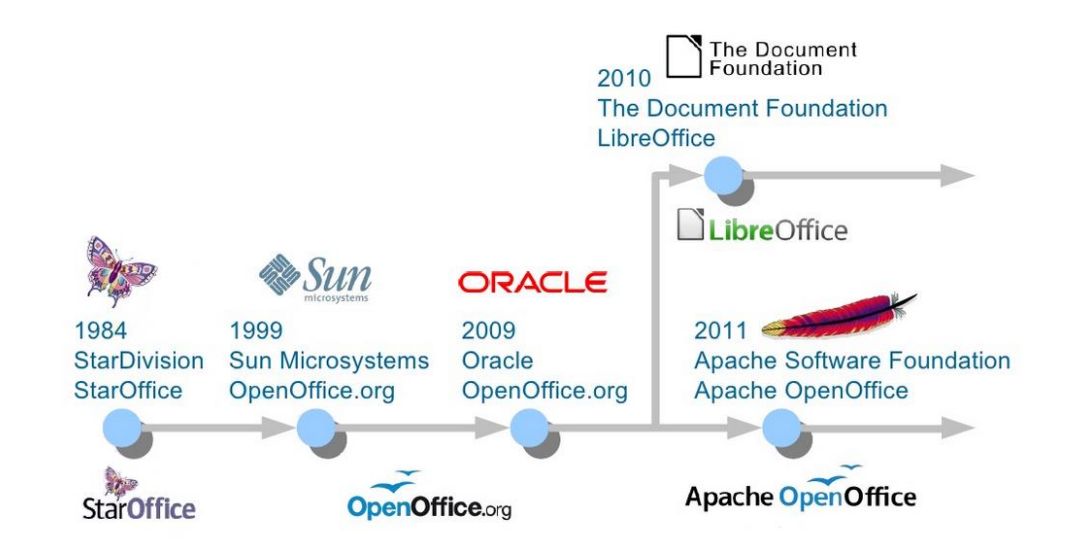
\includegraphics[width=13cm]{images/timeline.png}
	\caption{Timeline der Entwicklungsgeschichte}
	\label{timeline}
	
\end{figure}

\subsection{Generierungsvarianten}
\hon{}
Um ein \textit{Entity Relationship Diagramm} in \textit{LibreOffice Draw} automatisiert generieren zu können, bieten sich zwei Möglichkeiten an, die sich in der Komplexität und der Umsetzung sehr stark unterscheiden. Die erste der beiden Möglichkeiten ist der Zugriff über die zu Verfügung stehende \textit{API}. Die zweite Variante ist die Manipulation des Dateiformats.

\subsubsection{Generierung über die LibreOffice API}

\subsubsubsection{Allgemeines}
\hon{}
\\
\noindent
Um über die \textit{LibreOffice Programmierschnittstelle} (\textit{API}) auf ein \textit{Draw} Dokument zugreifen zu können benötigt man das \textit{LibreOffice Software Development Kit}. Dieses beinhaltet ein Set von Entwicklungswerkzeugen, Bibliotheken und Header-Dateien.
Auf der Website der \textit{LibreOffice} API befinden sich diverse Beispiele um die Funktionsweise und die Verwendung der \textit{API} zu demonstrieren. Die verschiedenen Beispiele unterscheiden sich in der verwendeten Programmiersprache und dem Zielprogramm. Als Programmiersprachen stehen \textit{Java, C++, Python, Basic} und das Objektsystem \textit{Object Linking and Embedding} zur Verfügung. Bei der genaueren Betrachtung zeigt sich, dass das einzige Beispiel, dass \textit{Draw} als Zielprogramm hat, in \textit{Java} geschrieben ist. 
\footfullcite[][]{LibreOfficeAPI}
\\
\hon{}
\\

\noindent
Um in ein \textit{Draw} Dokument zeichnen zu können, muss zuerst ein Dokument, eine Instanz der Klasse \verb|com.sun.star.frame.Desktop| mit einem Kontext der Klasse \verb|com.sun.star.uno.| \verb|XComponentContext| und einem \textit{Komponentenlader} mit der Instanz der Klasse \verb|com.sun.| \verb|star.frame.Desktop| angelegt werden. In der folgenden Grafik befindet sich ein Beispiel für jenen Code. (siehe Listing \ref{listing1})

\noindent
\hon{}
\lstset{language=Java}
\lstset{frame=lines}
\lstset{caption={Programmcode in Java, um ein leeres \textit{Draw} Dokument zu öffnen}}
\lstset{label={listing1}}
\lstset{basicstyle=\footnotesize}
\begin{lstlisting}

com.sun.star.frame.XComponentLoader xCLoader;
com.sun.star.lang.XComponent xComp = null;

try {
    com.sun.star.lang.XMultiComponentFactory xMCF = 
    xContext.getServiceManager();

    Object oDesktop = xMCF.createInstanceWithContext
    ("com.sun.star.frame.Desktop", xContext);

    xCLoader = UnoRuntime.queryInterface
    (com.sun.star.frame.XComponentLoader.class, oDesktop);
    com.sun.star.beans.PropertyValue szEmptyArgs[] = 
    new com.sun.star.beans.PropertyValue[0];
    String strDoc = "private:factory/sdraw";
    xComp = xCLoader.loadComponentFromURL
    (strDoc, "_blank", 0, szEmptyArgs);

} catch (java.lang.Exception e) {
    System.err.println(" Exception " + e);
    e.printStackTrace(System.err);
}
\end{lstlisting}
\footfullcite[][]{LibreOfficeAPI}

\noindent
\hon{}
\\
\noindent
Über einige weitere Schritte erhält man ein Objekt der Klasse \verb|xShapes|, in das man dann die zu zeichnenden Objekte hinzufügt. (siehe Listing \ref{listing2})
\noindent
\lstset{language=Java}
\lstset{frame=lines}
\lstset{caption={Programmcode in Java, um ein leeres \textit{Draw} Dokument zu öffnen}}
\lstset{label={listing2}}
\lstset{basicstyle=\footnotesize}
\begin{lstlisting}
xDrawDoc = openDraw(xContext);
try {
    System.out.println("getting Drawpage");
    com.sun.star.drawing.XDrawPagesSupplier xDPS = UnoRuntime
    .queryInterface(com.sun.star.drawing.
    XDrawPagesSupplier.class, xDrawDoc);
    com.sun.star.drawing.XDrawPages xDPn = xDPS.getDrawPages();
    com.sun.star.container.XIndexAccess xDPi = UnoRuntime
    .queryInterface(com.sun.star.container.XIndexAccess.class,
    xDPn);
    xDrawPage = UnoRuntime.queryInterface(com.sun.star.drawing.
    XDrawPage.class, xDPi.getByIndex(0));
} catch (java.lang.Exception e) {
    System.err.println("Couldn't create document" + e);
    e.printStackTrace(System.err);
}
\end{lstlisting}
\footnotemark[32]
\noindent
\\
\noindent
Mit dem in Listing \ref{listing1} und \ref{listing2} gezeigten Programmcode öffnet sich ein \textit{LibreOffice Draw} Dokument ohne Inhalt.

\noindent
\subsubsubsection{XERML-Daten Aufbereitung in Java}
\label{XERML-JAVA}
\hon{}

\noindent
Um die Daten aus der \textit{XERML}-Datei in ein für \textit{Java} interpretierbares Format zu bringen, wird der \textit{Java DOM Parser} verwendet. Die Daten werden immer in einer Liste des Datentyps \verb|ArrayList<String>| mit folgendem Aufbau gespeichert:
\begin{itemize}
	\item Für \textit{Entity-Typen} und zugehörige Attribute: Das erste Listenelement enthält den Namen des \textit{Entity-Typs}. Die folgenden Listenelemente enthalten die Namen der \textit{Attribute}.
	\item Für \textit{Beziehungstypen} und deren Teilnehmer: Das erste Listenelement enthält den Namen des \textit{Beziehungstyps}. Für jeden  Teilnehmer werden Listenelemente in folgender Reihenfolge hinzugefügt: Name des teilnehmenden \textit{Entity-Typs}, Minimalwert, Maximalwert.
	\item Für \textit{Beziehungsattribute}: Das erste Listenelement enthält den Namen des \textit{Beziehungstyps}. \textit{Beziehungsattribute} werden, falls vorhanden, dahinter angehängt.
	\item Für \textit{Primary-Keys}: Das erste Listenelement enthält den Namen des \textit{Entity-Typs}. Die darauffolgenden Listenelemente sind ein oder mehrere \textit{Primary-Keys}.
	\item Für \textit{Super-Sub-Beziehungstypen}: Das erste Listenelement enthält den Namen des \textit{Beziehungstyps}. Das zweite und dritte Listenelement enthalten den Wert des \textit{XERML-Attributs} \textit{total} an zweiter Stelle und den Wert des \textit{XERML-Attributs} \textit{disjunkt} an dritter Stelle. Dieser kann entweder \verb|true| oder \verb|false| sein. 
\end{itemize}


\noindent
\subsubsubsection{Darstellung der grafischen Elemente}
\hon{}

\noindent
Grundsätzlich folgt die Darstellung der verschiedenen grafischen Formen immer dem gleichen Schema. Zuerst wird ein Objekt, das die derzeitige Seite des Dokuments beinhaltet, angelegt. Dieses wird dann in ein Objekt der Klasse \verb|xDrawPage| umgewandelt. Parallel dazu benötigt man ein Objekt der Klasse \verb|XShape|, welches eine Vorlage beinhaltet. Die Vorlage bestimmt die Form des grafischen Elements. 


\noindent
\hon{}
\\
\noindent
Für die Erstellung der Komponenten eines \textit{ERDs} sind folgende Klassen notwendig:
\begin{itemize}
	\item \verb|RectangleShape| für die Erstellung von Rechtecken um  \textit{Entity-Typen} darzustellen.
	\item \verb|EllipseShape| für die Erstellung von Ellipsen um \textit{Attribute} darzustellen.
	\item \verb|PolyPolygonShape| für die Erstellung von Rauten und Dreiecken um \textit{Beziehungs-} und \textit{Super-Sub-Beziehungstypen} darzustellen. Die Klasse kann Formen mit einer beliebigen Anzahl an Seiten darstellen. 
	\item \verb|ConnectorShape| für die Erstellung von Linien, die \textit{Entity-Typen} mit \textit{Attributen} und \textit{Entity-Typen} mit \textit{Beziehungstypen} verbinden. Die Klasse \verb|LineShape| ermöglicht es lediglich die Endpunkte der Linie an eine bestimmte Koordinate zu binden. Falls, in der Nachbearbeitung, eine Form verschoben wird, bleibt die Linie an der festgelegten Koordinate. Um diesem Problem entgegen zu wirken, wird die Klasse \verb|ConnectorShape| verwendet, bei der man die Endpunkte der Linie an ein Objekt einer anderen Klasse binden kann. 
	\item \verb|XText| für die Erstellung von Textfeldern um die Namen der \textit{Entity-Typen} und der \textit{Attribute} anzuzeigen. Für die \textit{min-max-Notation} sind Textfelder ebenfalls nötig.
\end{itemize}
\footfullcite[][]{OpenOfficeDevelopersGuide}
\footfullcite[][]{LibreOfficeAPI}
\noindent
\hon{}
\\
\noindent
In allen oben gelisteten Klassen besteht die Möglichkeit, dem Objekt eine Position zuzuweisen. Wird keine Position explizit angegeben, so werden die Koordinaten [0,0] verwendet, wobei sich die Koordinaten auf den linken oberen Punkt des Objekts bezieht. 
\\
\noindent
Die Funktion \verb|setSize| der Klasse \verb|xDrawShape| setzt die Breite und Höhe der Form fest.
Standardmäßig werden die Objekte mit einem schwarzen Rand und weißer Füllung gezeichnet. 
\\
\noindent
Mit der Funktion \verb|setPropertyValue| der Klasse \verb|XPropertySet| kann man die Objekte in einer beliebigen Farbe darstellen. Die Farbwerte werden im Dezimalformat angegeben.
\\

\noindent
Die Listing \ref{listing3} zeigt den Programmcode um einen \textit{Entity-Typ} zu erstellen. Die Variablen \verb|x| und \verb|y| enthalten dabei die Koordinaten, wo das Rechteck gezeichnet werden soll. Die Variable \verb|col| enthält den Dezimalwert \textit{16711680}. Dies entspricht einer rötlichen Färbung. In der Variable \verb|text| wird der Name des \textit{Entity-Typs} mitgegeben, der in der Schriftgröße \textit{6pt} mittig in das Rechteck gezeichnet wird.

\noindent
\hon{}
\lstset{language=Java}
\lstset{frame=lines}
\lstset{caption={Programmcode in Java, um ein Entity-Typ mit Text in der Schriftgröße 6pt zu zeichnen}}
\lstset{label={listing3}}
\lstset{basicstyle=\footnotesize}
\begin{lstlisting}

Object drawPages = xDrawPagesSupplier.getDrawPages();
XIndexAccess xIndexedDrawPages = (XIndexAccess) 
UnoRuntime.queryInterface(XIndexAccess.class, drawPages);
Object drawPage = xIndexedDrawPages.getByIndex(0);
XMultiServiceFactory xDrawFactory = (XMultiServiceFactory) 
UnoRuntime.queryInterface(XMultiServiceFactory.class, xComponent);
Object drawShape = xDrawFactory.createInstance
("com.sun.star.drawing.RectangleShape");
XDrawPage xDrawPage = (XDrawPage) 
UnoRuntime.queryInterface(XDrawPage.class, drawPage);
xDrawShape = UnoRuntime.queryInterface(XShape.class, drawShape);
xDrawShape.setSize(new Size(width, height));
xDrawShape.setPosition(new Point(x, y));
xDrawPage.add(xDrawShape);

XText xShapeText = UnoRuntime.queryInterface(XText.class, 
drawShape);
XPropertySet xShapeProps = UnoRuntime.queryInterface
(XPropertySet.class, drawShape);

xShapeProps.setPropertyValue("FillColor", Integer.valueOf(col));

com.sun.star.text.XTextCursor xTCursor = xShapeText.
createTextCursor();
com.sun.star.beans.XPropertySet xTCPS = 
UnoRuntime.queryInterface(com.sun.star.beans.XPropertySet.class,
xTCursor);
xTCPS.setPropertyValue("CharHeight", 6.0f);
xShapeText.insertString(xTCursor, text, false);
com.sun.star.beans.XPropertySet xText = 
UnoRuntime.queryInterface(com.sun.star.beans.XPropertySet.class,
xShapeProps);

\end{lstlisting}
\noindent
\\
\noindent

\hon{}
\noindent
Das Ergebnis des Programmcodes angewendet auf das Weingut Testmodell wird in Abbildung \ref{ergebnis3} abgebildet:

\begin{figure}[h]
	\centering
	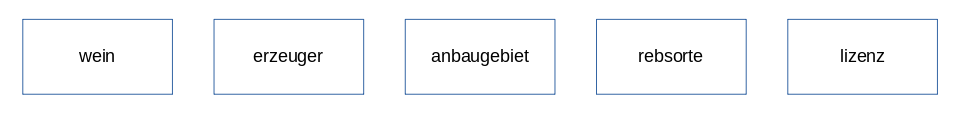
\includegraphics[width=14cm]{images/5.png}
	\caption{Erzeugte \textit{Entity-Typen} mittels Programmcode von Listing \ref{listing3} angewendet auf das Weingut Testmodell}
	\label{ergebnis3}
\end{figure}
\hon{}
\noindent
Die Erstellung der \textit{Attribute} erfolgt nahezu analog zu der Erstellung der \textit{Entity-Typen}. Anstatt der Klasse \verb|RectangleShape| ist die Klasse \verb|EllipseShape| zu verwenden. Falls das \textit{Attribut} ein \textit{Primary-Key} ist, wird der Name des \textit{Attributs} unterstrichen.
\noindent
\\
\\
\noindent
In Abbildung \ref{ergebnis4} sieht man die \textit{Attribute} des \textit{Entity-Typs} Wein: 


\begin{figure}[h]
	\centering
	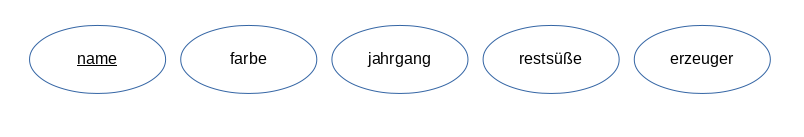
\includegraphics[width=14cm]{images/7.png}
	\caption{Erzeugte Attribute von dem Entity-Typ Wein des Weingut Testmodells}
	\label{ergebnis4}
\end{figure}

\hon{}
\noindent
Im Gegensatz zu Rechtecken oder Ellipsen gibt es keine vordefinierten Formen um \textit{Beziehungstypen} durch eine Raute oder \textit{Super-Sub-Beziehungstypen} durch ein gleichschenkeliges Dreieck darzustellen. An dieser Stelle kommt die Klasse \verb|PolyPolygonShape| zum Einsatz. Mithilfe dieser Klasse und den Funktionen aus Listing \ref{listing5} kann eine Form mit einer beliebigen Anzahl an Seiten erzeugt werden.

\lstset{language=Java}
\lstset{frame=lines}
\lstset{caption={Programmcode in Java, um einen Rechteck mit beliebiger Anzahl an Eckpunkten zu erzeugen}}
\hon{}
\lstset{label={listing5}}
\lstset{basicstyle=\footnotesize}
\begin{lstlisting}
public static XShape drawPolygon(XDrawPage slide, int x, int y, int radius, int nSides, String text) {
    XShape polygon = addShape(slide, "PolyPolygonShape", 0, 0, 0, 0, text);
    Point[] pts = genPolygonPoints(x, y, radius, nSides);
    Point[][] polys = new Point[][] { pts };
    setProperty(polygon, "PolyPolygon", polys);
    return polygon;
}

public static XShape addShape(XDrawPage slide, String shapeType, int x, int y, int width, int height, String text) {
    XShape shape = makeShape(shapeType, x, y, width, height, text);
    if (shape != null){
        slide.add(shape);
    }
    return shape;
}

public static XShape makeShape(String shapeType, int x, int y, int width, int height, String text) {
    XShape shape = null;
    try {
        shape = createInstanceMSF(XShape.class, "com.sun.star.drawing." + shapeType);
        shape.setPosition(new Point(x * 100, y * 100));
        shape.setSize(new Size(width * 100, height * 100));
    } catch (java.lang.Exception e) {
        System.out.println("Unable to create shape: " + shapeType);
    }
    return shape;
}

private static Point[] genPolygonPoints(int x, int y, int radius, int nSides) {
    if (nSides < 3) {
        System.out.println("Too few sides; must be 3 or more");
        nSides = 3;
    } else if (nSides > 30) {
        System.out.println("Too many sides; must be 30 or less");
        nSides = 30;
    }

    Point[] pts = new Point[nSides];
    double angleStep = Math.PI / nSides;
    for (int i = 0; i < nSides; i++) {
        pts[i] = new Point((int) Math.round(x * 100 + radius * 100 * Math.cos(i * 2 * angleStep)),
        (int) Math.round(y * 100 + radius * 100 * Math.sin(i * 2 * angleStep)));
    }
    return pts;
}
\end{lstlisting}
\footfullcite[][]{JavaLibreOfficeProgramming}
\noindent
\\
\hon{}
\\
\noindent
Durch den Aufruf der Funktion \verb|drawPolygon| aus dem Listing \ref{listing5}, die die anderen Funktionen aus dieser Listing aufruft, wird ein Polygon erzeugt. Die Parameter der Funktion haben folgende Bedeutung:
\begin{itemize}
	\item \verb|XDrawPage slide|: beinhaltet die Seite in die das \textit{Polygon} gezeichnet wird.
	\item \verb|int x|: legt den Wert der x-Koordinate fest.
	\item \verb|int y|: legt den Wert der y-Koordinate fest.
	\item \verb|int radius|: legt die Größe der zu zeichnenden Form fest.
	\item \verb|int nSides|: legt die Seitenanzahl der Form fest. Dieser Wert muss zwischen exklusive drei und exklusive dreißig liegen.
	\item \verb|String text|: beinhaltet den Text, der in der Form angezeigt wird.  
\end{itemize}

\noindent
\hon{}
\\
\noindent
Das Ergebnis der Aufrufe \\
\verb|drawPolygon(xDrawPage, 10, 10, 8, 4, "erzeugt");| 
\\ \verb|drawPolygon(xDrawPage, 20, 10, 8, 4, "beinhaltet");| \\ \verb|drawPolygon(xDrawPage, 30, 10, 8, 3, "");| \\
ist in Abbildung \ref{ergebnis5} dargestellt.

\begin{figure}[h]
	\centering
	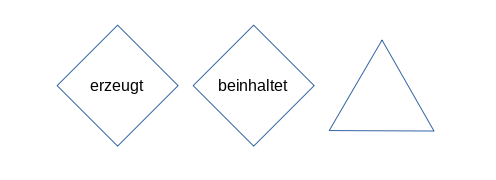
\includegraphics[width=8cm]{images/8.png}
	\caption{Zwei Beziehungstypen und ein Super-Sub-Beziehungstyp}
	\label{ergebnis5}
\end{figure}

\hon{}
\noindent
Um einen \textit{Entity-Typ} mit einem \textit{Beziehungstyp} oder einem \textit{Attribut} zu verbinden, wird die Klasse \verb|XPropertySet| benötigt. Dieser Klasse wird ein Objekt der Klasse \verb|ConnectorShape| mitgegeben. Der Programmcode aus Listing \ref{listing6} zeigt, wie man zwei \textit{Konnektoren} erzeugt und diese von dem \textit{Beziehungstyp} zu zwei verschiedenen \textit{Entity-Typen} verbindet:


\noindent
\lstset{language=Java}
\lstset{frame=lines}
\lstset{caption={Programmcode in Java, um zwei \textit{Konnektoren} zu erzeugen und von einem \textit{Beziehungstyp} zu zwei verschiedenen \textit{Entity-Typen} zu binden}}
\lstset{label={listing6}}
\lstset{basicstyle=\footnotesize}
\begin{lstlisting}

XPropertySet xConnector1PropSet = (XPropertySet) 
UnoRuntime.queryInterface(XPropertySet.class, connector1);
XPropertySet xConnector2PropSet = (XPropertySet) 
UnoRuntime.queryInterface(XPropertySet.class, connector2);

xConnector1PropSet.setPropertyValue("StartShape", diamond);
xConnector1PropSet.setPropertyValue("EndShape", start_shape);
xConnector2PropSet.setPropertyValue("StartShape", diamond);
xConnector2PropSet.setPropertyValue("EndShape", end_shape);

\end{lstlisting}
\noindent
\\
\noindent
Das Ergebnis aus Listing \ref{listing6} wird in Abbildung \ref{ergebnis6} dargestellt.
\begin{figure}[H]
	\centering
	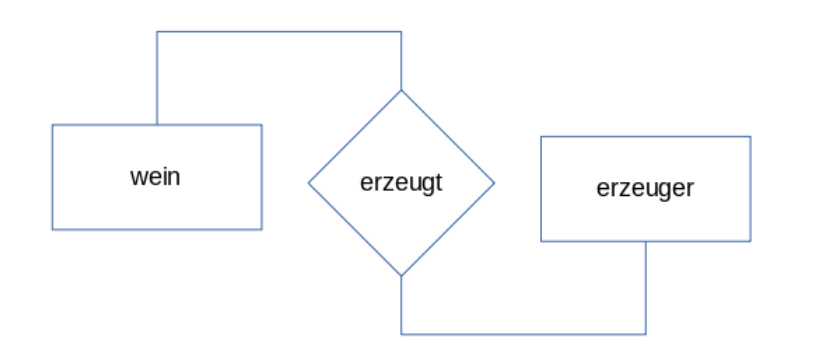
\includegraphics[width=8cm]{images/11.png}
	\caption{Ergebnis aus Listing 4}
	\label{ergebnis6}
\end{figure}
\noindent
Während der Entwicklung über die \textit{API} sind einige Probleme wie zum Beispiel das korrekte Darstellen von \textit{Konnektoren} und \textit{abhängigen Entity-Typen} aufgetreten, weshalb die Weiterentwicklung der Darstellung von \textit{ERDs} über die \textit{API} eingestellt wurde.



\subsubsubsection{Vor- und Nachteile}
\hon{}
\\
Die \textit{LibreOffice API} bietet eine Variante, um ein \textit{LibreOffice}-Dokument zu bearbeiten ohne Modifikationen am Dateiformat vorzunehmen. Dies ist aber nicht der einzige Vorteil:
\begin{itemize}
	\item Die \textit{LibreOffice API} ist zu 100 Prozent kompatibel mit \textit{OpenOffice}. Das bedeutet einerseits, dass das Zielprogramm sowohl ein \textit{LibreOffice} Programm als auch ein \textit{OpenOffice} Programm sein kann, und andererseits, dass es dem Anwendungsprogrammierer frei steht, welche Dokumentation er wählt. 
	\item Darüber hinaus ist sowohl die \textit{LibreOffice API} Dokumentation als auch die \textit{OpenOffice API} Dokumentation sehr umfangreich.
\end{itemize}
\footfullcite[][]{OpenOfficeDevelopersGuide}
\noindent
\\
\noindent
Allerdings bringt diese Methode auch einige Nachteile mit sich:
\\
\begin{itemize}
	\item Die Dokumentation erstreckt sich über 1650 Seiten, was einen einfachen Einstieg in die \textit{API} sehr schwierig macht.
	\item Des Weiteren ist die Dokumentation sehr unübersichtlich und unstrukturiert gestaltet. 
	\item Die Nummerierung der Kapitel und Unterkapitel ist in der Dokumentation nicht angegeben.
	\item Die letzte Version der Dokumentation ist 2009 erschienen und somit veraltet.
	\item Es gibt trotz der langen Entwicklungsgeschichte von \textit{OpenOffice} beziehungsweise \textit{LibreOffice} wenige Anwendungsbeispiele, was ein Erlernen allein durch den Programmcode schwierig gestaltet.
	\item Die Generierung von \textit{ERDs} über die \textit{API} ist ressourcenintensiver und dauert länger als die Generierung über das Dateiformat.
	\item Selbst bei der einfachen Verwendung der \textit{API} müssen oft viele Klassen und Konvertierungen zwischen Klassen erfolgen, um das gewünschte Ergebnis zu erhalten, was das Benutzen der \textit{API} ebenfalls erschwert.   
	\item Viele Objekte, die man in \textit{LibreOffice Draw} händisch erzeugen kann, sind in der \textit{API} nicht vorhanden, wie zum Beispiel ein Dreieck oder eine Raute. Diese müssen dann aufwendig durch die Klasse \verb|PolyPolygonShape| erstellt werden, was einen höheren Programmieraufwand mit sich bringt.
	\item Um die \textit{API} verwenden zu können, ist das \textit{LibreOffice Software Development Kit} notwendig. Dieses muss in jeder Sitzung ausgeführt werden, was Performanceeinbußen mit sich bringt.
\end{itemize}
\footfullcite[][]{OpenOfficeDevelopersGuide}

\noindent
\subsubsection{Generierung über das Dateiformat}
\hon{}



\subsubsubsection{Allgemeines}

\noindent	
\textit{LibreOffice Draw} verwendet das \textit{Open Document Graphics} (ODG) Dateiformat, das 2006 als internationale Norm ISO/IEC 26300 veröffentlicht wurde. 
\textit{ODG} basiert auf einem \textit{XML-Vokabular}, dessen Elemente an den Standard HTML angelehnt sind.
Eine \textit{OpenDocument}-Datei besteht aus einer Sammlung mehrerer \textit{XML-Dateien} und anderer Objekte wie Bilder oder Thumbnails, die zu einer Datei im ZIP-Format zusammengefasst werden.
\\
Bei der Entpackung dieser ZIP-Datei sieht man folgende Dateien und Ordner:
\begin{verbatim}
Datei.odt
|
+-- META-INF
|    |
|    +-- manifest.xml
|
+-- Thumbnails
|    |
|    +-- thumbnail.png
|
+-- Pictures
|    |
|    +-- picture.png
|
+-- mimetype
+-- content.xml
+-- styles.xml
+-- meta.xml
+-- settings.xml
\end{verbatim}
\footfullcite[][]{LibreOfficeWikipedia}

\noindent
Inhalt dieser Dateien:
\hon{}
\begin{itemize}
	\item  \textit{manifest.xml}: In dieser Datei befindet sich eine Übersicht aller Dateien mit deren Pfaden und zulässigen Datentypen.
	\item \textit{thumbnail.png}: Diese Datei zeigt eine Miniaturansicht der ersten Seite des Dokuments.
	\item Im Pictures-Ordner befinden sich alle eingebundenen Bilder des Dokuments. Falls keine Bilder eingebunden sind, existiert dieser Ordner nicht. 
	\item \textit{mimetype}: Diese Datei ist eine Textdatei, deren einziger Inhalt eine Zeile mit dem Typ der \textit{LibreOffice}-Datei ist. Beim Beispiel einer \textit{Draw}-Datei steht folgender Inhalt in der \textit{Mimetype}-Datei: 
	\\
	\verb|application/vnd.oasis.opendocument.graphics|
	\item \textit{settings.xml}: In dieser Datei befinden sich sämtliche \\ Einstellungsmöglichkeiten, die \textit{LibreOffice Draw} anbietet. Darunter fallen zum Beispiel die Maßeinheit, Name und Setup der Drucker, die Skalierung und die Sichtbarkeit der einzelnen Ebenen.
	\item \textit{content.xml}: In dieser Datei befindet sich der eigentliche Inhalt des Dokuments. Durch Betrachtung einer \textit{Draw}-Datei ohne Inhalt ergibt sich die Baumstruktur:
	\begin{verbatim}
	Element: office:document-content
	|
	+-- Attribut: xmlns:--
	+-- Element: office:scripts
	+-- Element: office:font-face-decls
	    |
	    +-- Element: style:font-face
	        |
	        +-- Attribut: style:name
	        +-- Attribut: style:font-family
	        +-- Attribut: style:font-family-generic
	        +-- Attribut: style:font-pitch
	        +-- Element: office:automatic-styles
	            |
	            +-- Element: style:style
	                |
	                +-- Attribut: style:name
	                +-- Attribut: style:family
	                +-- Element: office:body
	                    |
	                    +-- Element: office:drawing
	                        |
	                        +-- Element: draw:page
	                            |
	                            +-- Attribut: draw:name
	                            +-- Attribut: draw:style-name
	                            +-- Attribut: draw:master-page-name
	\end{verbatim}
	
	\noindent
	\hon{}
	\\
	\noindent
	Der komplette Inhalt wird als \textit{XML-Kindelement} von dem \textit{XML-Element} \verb|draw:page| eingefügt.
	In dem \textit{XML-Element} \verb|office:document-content| befinden sich mehrere \textit{XML-Attribute} mit diversen \textit{Namensräumen}, die aus Gründen der \\ Übersichtlichkeit weggelassen wurden.
	
	\item \textit{styles.xml}: Diese Datei beinhaltet die grafischen Informationen der Formatvorlagen für Texte und grafischen Elemente wie zum Beispiel Textfarbe, Textgröße, Füllungsfarbe, Abstand an den Seiten, Rahmenbreite, etc. 
	\item \textit{meta.xml}: In dieser Datei befinden sich Übersichtsinformationen der \textit{LibreOffice}-Datei wie zum Beispiel der Name des Erzeugers, das Datum, an dem das Dokument erstellt wurde, die Sprache des Dokuments und die Bearbeitungsdauer.
	
\end{itemize}
\footfullcite[][]{LibreOfficeWikipedia}
\noindent
\hon{}
\\
\noindent
Wie man in der obigen Auflistung sieht, ist das Dateiformat \textit{ODG} komplex und daher aufwändig zu modifizieren.
\textit{LibreOffice} bietet allerdings auch die Möglichkeit eine \textit{Draw}-Datei in dem Dateiformat \textit{Flat Open Document Graphics} (\textit{FODG}) zu speichern. In diesem Format werden die Dateien aus dem gezippten Ordner zu einer Datei zusammengefasst. Diese Variante der Speicherung ist für die Manipulation des Dateiformats am besten geeignet, da nur eine einzige Datei manipuliert werden muss. 
Für die Manipulation über das Dateiformat wird die Programmiersprache \textit{Python} verwendet. Diese bringt im Zusammenhang mit der gewählten Diplomarbeit mehrere Vorteile mit sich:
\begin{itemize}
	\item In der Regel ist es einfacher und schneller kleinere Programme wie diese Diplomarbeit in \textit{Python} zu entwickeln.
	\item \textit{Python} ist eine plattformunabhängige Sprache, die auf fast allen Betriebssystemen vorhanden ist. 
\end{itemize}

\subsubsubsection{XERML-Daten Aufbereitung in Python}
\hon{}

\noindent
In der Programmiersprache \textit{Python} gibt es mehrere Optionen eine \textit{XML-Datei} zu \textit{parsen} und dessen Daten in ein geeignetes Format für die Weiterverarbeitung zu bringen. Im Zuge der Diplomarbeit ist die Entscheidung auf \textit{LXML} gefallen. \textit{LXML} ist eine \textit{Python}-Bibliothek und bietet einen sicheren und bequemen Zugriff auf die \textit{libxml2} und \textit{libxslt} Bibliothek mithilfe der \textit{ElementTree API}. Die Daten aus der \textit{XML-Datei} werden in einem Array mit dem selben Aufbau wie in Kapitel \ref{XERML-JAVA} gespeichert.


\subsubsubsection{Darstellung der grafischen Elemente}

\noindent
\textbf{Alle Annahmen und Informationen dieses Kapitels entstammen keiner Quelle und wurden durch \textit{Reverse Engineering} in Erfahrung gebracht.}

\hon{}
\noindent
\\
\noindent
Bei jeden Aufruf ein komplettes \textit{LibreOffice} Dokument zu generieren, bedeutet viel Programmieraufwand und beeinträchtigt die Performance. Aus diesem Grund wird das zuvor erstellte leere \textit{LibreOffice} Dokument \textit{empty1.fodg} als Ausgangsdokument verwendet. Um das Dokument auf die Darstellung von \textit{ERDs} zu optimieren, wurden kleinere Modifikationen vorgenommen:
\begin{itemize}
	\item Das Dokument hat einen \textit{Margin} von 1.9 cm.
	\item Sämtliche \verb|gr|, \verb|t| und \verb|p| \textit{XML-Elemente} wurden angepasst. 
	\item Die Informationen über das Format, die Breite und die Höhe wurden entfernt.
\end{itemize} 
\noindent
\hon{}
\\
\noindent
Sämtliche grafische Formen lassen sich mit dem \textit{XML-Element} \verb|custom-shape| erzeugen. Dafür muss man das \textit{XML-Element} als \textit{XML-Kindelement} von dem \textit{XML-Element} \verb|draw:page| einfügen. Das \textit{XML-Element} \verb|custom-shape| benötigt ebenfalls zwei \textit{XML-Kindelemente} um den Text in der grafischen Form anzuzeigen und um die grafischen Eigenschaften der Form festzulegen. Der Aufbau der \textit{XML-Elemente} und deren \textit{XML-Attribute} bei der Erstellung von Rechtecken für \textit{Entity-Typen} und Ellipsen für \textit{Attribute} sieht wie folgt aus:

\begin{verbatim}
Element: draw:page
|
+-- Element: draw:custom-shape
    |
    +-- Attribut: draw:style-name
    +-- Attribut: draw:text-style-name
    +-- Attribut: draw:id
    +-- Attribut: draw:layer
    +-- Attribut: svg:width
    +-- Attribut: svg:height
    +-- Attribut: svg:x
    +-- Attribut: svg:y
    +-- Element: draw:enhanced-geometry
        |
        +-- Attribut: svg:viewBox
        +-- Attribut: draw:mirror-horizontal
        +-- Attribut: draw:mirror-vertical
        +-- Attribut: draw:type
        +-- Attribut: draw:enhanced-path
        +-- Attribut: svg:glue-points
        +-- Attribut: draw:text-areas
        +-- Element: text:p
            |
            +-- Attribut: text:style-name
            +-- Element: text:span
                |
                +-- Attribut: text:style-name

\end{verbatim}
\hon{}
\noindent
Einige der \textit{XML-Attribute} sind für die Erstellung eines \textit{ERDs} unrelevant beziehungsweise werden immer mit den selben Werten befüllt:
\begin{itemize}
	\item Das Attribut \verb|draw:layer| beschreibt die Ebene der Form. Das Ausgangsdokument beinhaltet folgende Ebenen: \textit{layout}, \textit{background}, \textit{backgroundobjects}, \textit{controls} und \textit{measurelines}. Die Ebenen sind absteigend in Richtung Hintergrund geordnet.
	Für die Erstellung eines \textit{ERDs} sind mehrere Ebenen nicht vorgesehen, weshalb dem \textit{XML-Attribut} \verb|draw:layer| immer der Wert \textit{layout} zugeordnet wird.
	\item Mit dem \textit{XML-Attribut} \verb|svg:viewBox| wird eine fixe Pixelbreite und Pixelhöhe festgelegt. Dem Attribut wird immer der Wert \verb|0 0 21600 21600| zugewiesen. 
	\item Die \textit{XML-Attribute} \verb|draw:mirror-horizontal| und \verb|draw:mirror-vertical| bekommen den Wert \verb|false| zugewiesen. 
	\item Das \textit{XML-Attribut} \verb|draw:enhanced-path| bekommt den Wert \verb|U 10800 10800 10800| \verb| 10800 0 360 Z N|.
	\item Das \textit{XML-Attribut} \verb|svg:glue-points| legt die Klebepunkte der Form fest, an denen sich \textit{Konnektoren} anheften können. Diese haben den Wert \verb|10800 0 3163 3163 0| \verb|10800 3163 18437 10800 21600 18437 18437 21600 10800 18437 3163|.
	\item Das \textit{XML-Attribut} \verb|draw:text-areas| bekommt den Wert \verb|3163 3163 18437 18437|.
\end{itemize}
\noindent
\hon{}
\\
\noindent
Der Text wird unter \textit{LXML} mithilfe der Methode \verb|text| bei dem \textit{XML-Element} \verb|text:span| festgelegt.
Das \textit{ERD} kann mit Farbe oder farblos gezeichnet werden. 
Bei einer Darstellung in Farbe werden die Hexadezimalwerte \verb|89D8D6| für \textit{Entity-Typen}, \verb|89BED8| für \textit{Attribute} und \verb|93D889| für \textit{Beziehungstypen} verwendet.
\\
\hon{}

\noindent
Sämtliche Informationen über das Aussehen der Formen werden in den \textit{XML-Elementen} \verb|style:style| gespeichert. Es gibt drei verschiedene Kategorien. Die \verb|gr| \textit{XML-Elemente} speichern die grafischen Informationen. Die \textit{XML-Elemente} \verb|p| und \verb|t| speichern Informationen über die Darstellung von Text. Ein \verb|gr| \textit{XML-Element} könnte wie folgt aussehen:

\begin{verbatim}
<style:style style:name="gr1" style:family="graphic" 
       style:parent-style-name="standard">
    <style:graphic-properties svg:stroke-width="0.03cm" 
           svg:stroke-color="#000000" draw:marker-start-width="0.245cm"
           draw:marker-end-width="0.245cm" draw:fill="solid" 
           draw:fill-color="#ffffff"
           draw:textarea-horizontal-align="justify" 
           draw:textarea-vertical-align="middle"
           draw:auto-grow-height="false" fo:padding-top="0.14cm"
           fo:padding-bottom="0.14cm" fo:padding-left="0.265cm"
           fo:padding-right="0.265cm" style:protect="size"/>
</style:style>
\end{verbatim}
\noindent
\hon{}
\\
\noindent
Um \textit{Entity-Typen} darzustellen, muss das \textit{XML-Attribut} \verb|draw:type| des \textit{XML-Elements} \verb|draw:enhanced-geometry| den Wert \textit{rectangle} beinhalten. Falls die Darstellung in Farbe erwünscht ist, bekommen die \textit{XML-Attribute} die Werte aus der Tabelle \ref{tbl:beispieltabelle1}.
\begin{table}[h]
	\centering
	\begin{tabular}{lll}
		\textbf{Element} & \textbf{Attribut}  & \textbf{Wert} \\
		\\
		draw:custum-shape & draw:style-name           & gr-ent             \\
		draw:custum-shape & draw:text-style-nam      & P-ent             \\
		text:p & text:style-name       & P1             \\
		text:span & text:style-name       & T6             \\
		\\
	\end{tabular}
	
	\caption{Tabelle der \textit{XML-Attributwerte} um \textit{Entity-Typen} farbig darzustellen}
	\label{tbl:beispieltabelle1}
	% Verweis im Text mittels \ref{tbl:beispieltabelle}
	
\end{table}
\noindent
\hon{}
\\

\noindent
Ist ein Darstellen in Farbe nicht erwünscht, bekommen die \textit{XML-Attribute} die Werte aus Tabelle \ref{tbl:beispieltabelle2}

\begin{table}[H]
	\centering
	\begin{tabular}{lll}
		\textbf{Element} & \textbf{Attribut}  & \textbf{Wert} \\
		\\
		draw:custum-shape & draw:style-name           & gr1             \\
		draw:custum-shape & draw:text-style-nam      & P8             \\
		text:p & text:style-name       & P1             \\
		text:span & text:style-name       & T1             \\
		\\
	\end{tabular}
	
	\caption{Tabelle der \textit{XML-Attributwerte} um \textit{Entity-Typen} farblos darzustellen}
	\label{tbl:beispieltabelle2}
	% Verweis im Text mittels \ref{tbl:beispieltabelle}
	
\end{table}

\noindent
Die Breite und Höhe des Rechtecks werden in den \textit{XML-Attributen} \verb|svg:width| und \\ \verb|svg:height| festgelegt. Die Breite ist auf 10 cm und die Höhe ist auf 6 cm festgelegt.
\\
\noindent
Ein \textit{Entity-Typ} könnte in dem Dateiformat \textit{FODG} wie folgt aussehen:
\begin{verbatim}
<draw:custom-shape draw:style-name="gr_ent" draw:text-style-name="P_ent" 
      draw:id="wein" draw:layer="layout" svg:width="10cm" 
      svg:height="6cm" svg:x="159.6cm" 
      svg:y="82.73200000000001cm">
    <text:p text:style-name="P1">
        <text:span text:style-name="T6">wein</text:span>
    </text:p>
    <draw:enhanced-geometry svg:viewBox="0 0 21600 21600" 
          draw:mirror-horizontal="false" 
          draw:mirror-vertical="false" 
          draw:type="rectangle" 
          draw:enhanced-path="M 0 0 L 21600 0 21600 21600 0 21600 0 0 Z N" />
</draw:custom-shape>
\end{verbatim}
\noindent
\hon{}
\\
\noindent
In Abbildung \ref{ergebnis7} ist links das Ergebnis aus dem oben abgebildeten \textit{FODG} zu sehen und rechts ein \textit{Entity-Typ} ohne Farbe.
\begin{figure}[H]
	\centering
	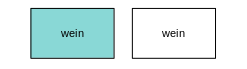
\includegraphics[width=7cm]{images/13.png}
	\caption{Links: Farbiger Entity-Typ in \textit{LibreOffice Draw}. Rechts: Farbloser Entity-Typ in \textit{LibreOffice Draw}}
	\label{ergebnis7}
\end{figure}
\noindent

\hon{}
\noindent
Die Darstellung von \textit{Attributen} funktioniert analog bis auf den Unterschied, dass das \textit{XML-Attribut} \verb|draw:type| den Wert \verb|ellipse| beinhaltet.
Falls ein Darstellen in Farbe erwünscht, bekommen die \textit{XML-Attribute} die Werte aus Tabelle \ref{tbl:beispieltabelle3}.

\begin{table}[H]
	\centering
	\begin{tabular}{lll}
		\textbf{Element} & \textbf{Attribut}  & \textbf{Wert} \\
		\\
		draw:custum-shape & draw:style-name           & gr4             \\
		draw:custum-shape & draw:text-style-nam      & P19             \\
		text:p & text:style-name       & P1             \\
		text:span & text:style-name       & T6            \\
		\\
	\end{tabular}
	
	\caption{Tabelle der \textit{XML-Attributwerte} um \textit{Attribute} farbig darzustellen}
	\label{tbl:beispieltabelle3}
	% Verweis im Text mittels \ref{tbl:beispieltabelle}
	
\end{table}
\hon{}
\noindent
Ist ein Darstellen in Farbe nicht erwünscht, bekommen die \textit{XML-Attribute} die Werte aus Tabelle \ref{tbl:beispieltabelle4}.

\begin{table}[H]
	\centering
	\begin{tabular}{lll}
		\textbf{Element} & \textbf{Attribut}  & \textbf{Wert} \\
		\\
		draw:custum-shape & draw:style-name           & gr1             \\
		draw:custum-shape & draw:text-style-nam      & P8            \\
		text:p & text:style-name       & P1             \\
		text:span & text:style-name       & T1             \\
		\\
	\end{tabular}
	
	\caption{Tabelle der \textit{XML-Attributwerte} um \textit{Attribute} farblos darzustellen}
	\label{tbl:beispieltabelle4}
	% Verweis im Text mittels \ref{tbl:beispieltabelle}
	
\end{table}

\noindent
Ein \textit{Attribut} könnte in dem Dateiformat \textit{FODG} wie folgt aussehen:
\begin{verbatim}
<draw:custom-shape draw:style-name="gr4" draw:text-style-name="P5" 
      draw:id="weinname" draw:layer="layout" svg:width="10cm" 
      svg:height="6cm" svg:x="182.76cm" svg:y="69.76cm">
    <text:p text:style-name="P1">
         <text:span text:style-name="T4">name</text:span>
    </text:p>
    <draw:enhanced-geometry svg:viewBox="0 0 21600 21600" 
          svg:glue-points="10800 0 3163 3163 0 10800 3163 18437 10800 
                           21600 18437 18437 21600 10800 18437 3163"
          draw:type="ellipse" draw:text-areas="3163 3163 18437 18437" 
          draw:enhanced-path="U 10800 10800 10800 10800 0 360 Z N" />
</draw:custom-shape>
\end{verbatim}

\hon{}
\noindent
Falls ein \textit{Attribut} ein \textit{Primary-Key} ist, wird der Name des \textit{Attributs} unterstrichen. Folgende Verwendung von \textit{XML-Attributen} ist dazu notwendig. 
Die \textit{XML-Attribute} bekommen die Werte aus Tabelle \ref{tbl:beispieltabelle5}, falls ein Darstellen in Farbe erwünscht ist.


\begin{table}[H]
	\centering
	\begin{tabular}{lll}
		\textbf{Element} & \textbf{Attribut}  & \textbf{Wert} \\
		\\
		draw:custum-shape & draw:style-name           & gr4             \\
		draw:custum-shape & draw:text-style-nam      & P5             \\
		text:p & text:style-name       & P1             \\
		text:span & text:style-name       & T4            \\
		\\
	\end{tabular}
	
	\caption{Tabelle der \textit{XML-Attributwerte} um \textit{Primary-Key-Attribute} in Farbe darzustellen}
	\label{tbl:beispieltabelle5}
	% Verweis im Text mittels \ref{tbl:beispieltabelle}
	
\end{table}
\noindent
\hon{}
\\
\noindent
Falls die Darstellung in Farbe nicht erwünscht ist, bekommen die \textit{XML-Attribute} die Werte aus Tabelle \ref{tbl:beispieltabelle6}.

\begin{table}[H]
	\centering
	\begin{tabular}{lll}
		\textbf{Element} & \textbf{Attribut}  & \textbf{Wert} \\
		\\
		draw:custum-shape & draw:style-name           & gr1             \\
		draw:custum-shape & draw:text-style-nam      & P7            \\
		text:p & text:style-name       & P1             \\
		text:span & text:style-name       & T4             \\
		\\
	\end{tabular}
	
	\caption{Tabelle der \textit{XML-Attributwerte} um \textit{Primary-Key-Attribute} farblos darzustellen}
	\label{tbl:beispieltabelle6}
	% Verweis im Text mittels \ref{tbl:beispieltabelle}
	
\end{table}
\hon{}
\noindent
In Abbildung \ref{ergebnis8} ist links außen ein farbiges \textit{Attribut} zu sehen, links mittig ein farbiges \textit{Primary-Key-Attribut}, rechts mittig ein \textit{Attribut} ohne Farbe und rechts außen ein farbloses \textit{Primary-Key-Attribut}:
\begin{figure}[H]
	\centering
	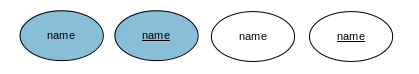
\includegraphics[width=12cm]{images/15.png}
	\caption{Links außen: Farbiges \textit{Attribut}. Links innen: Farbiges \textit{Primary-Key-Attribut}. Rechts innen: Farbloses \textit{Attribut}. Rechts außen: Farbloses \textit{Primary-Key-Attribut}}
	\label{ergebnis8}
\end{figure}
\hon{}
\noindent
Für die Darstellung von Rauten, um \textit{Beziehungstypen} darzustellen, benötigt das \textit{XML-Attribut} \verb|draw:type| den Wert \verb|diamond|. 
Falls ein Darstellen in Farbe erwünscht, bekommen die \textit{XML-Attribute} die Werte aus Tabelle \ref{tbl:beispieltabelle7}.


\begin{table}[H]
	\centering
	\begin{tabular}{lll}
		\textbf{Element} & \textbf{Attribut}  & \textbf{Wert} \\
		\\
		draw:custum-shape & draw:style-name           & gr-rel             \\
		draw:custum-shape & draw:text-style-nam      & P-rel             \\
		text:p & text:style-name       & P1             \\
		text:span & text:style-name       & T6            \\
		\\
	\end{tabular}
	
	\caption{Tabelle der \textit{XML-Attributwerte} um \textit{Beziehungstypen} farblos darzustellen}
	\label{tbl:beispieltabelle7}
	% Verweis im Text mittels \ref{tbl:beispieltabelle}
	
\end{table}
\hon{}
\noindent
Ist die Darstellung in Farbe nicht erwünscht ist, bekommen die \textit{XML-Attribute} die Werte aus Tabelle \ref{tbl:beispieltabelle8}.

\begin{table}[H]
	\centering
	\begin{tabular}{lll}
		\textbf{Element} & \textbf{Attribut}  & \textbf{Wert} \\
		\\
		draw:custum-shape & draw:style-name           & gr1             \\
		draw:custum-shape & draw:text-style-nam      & P8            \\
		text:p & text:style-name       & P1             \\
		text:span & text:style-name       & T1             \\
		\\
	\end{tabular}
	
	\caption{Tabelle der \textit{XML-Attributwerte} um \textit{Beziehungstypen} farblos darzustellen}
	\label{tbl:beispieltabelle8}
	% Verweis im Text mittels \ref{tbl:beispieltabelle}
	
\end{table}
\noindent
\textit{Konnektoren} lassen sich mit dem \textit{XML-Element} \verb|draw:connector| erzeugen.
Um die \textit{Konnektoren} mit einer Start- und Endform verbinden zu können und Text auf dem \textit{Konnektor} darzustellen, wird folgender Aufbau des Elements benötigt:
\begin{verbatim}
Element: draw:page
|
+-- Element: draw:connector
    |
    +-- Attribut: draw:style-name
    +-- Attribut: draw:text-style-name
    +-- Attribut: draw:id
    +-- Attribut: draw:layer
    +-- Attribut: draw:type
    +-- Attribut: start-shape
    +-- Attribut: end-shape
    +-- Attribut: svg:d
    +-- Attribut: svg:viewBox
    +-- Element: text:p
        |
        +-- Attribut: text:style-name
        +-- Element: text:span
            |
            +-- Attribut: text:style-name

\end{verbatim}
\hon{}
\noindent
Die \textit{XML-Attribute} \verb|draw:start-shape| und \verb|draw:end-shape| legen dabei die Start- und Endform fest, wobei sie als Wert die ID der zu verbindenden Form bekommen. Der Text, der auf dem \textit{Konnektor} steht, wird wie bei einem \textit{Entity-Typen} festgelegt. 
\noindent
Ein \textit{Konnektor}, der von einem \textit{Entity-Typ} zu einem \textit{Beziehungstyp} führt, könnte in dem Dateiformat \textit{FODG} wie folgt aussehen:

\begin{verbatim}
<draw:connector draw:style-name="gr2" draw:text-style-name="P3"
      draw:layer="layout" draw:type="line" 
      draw:start-shape="beinhaltet" 
      draw:end-shape="wein" 
      svg:d="M21575 3050l2125 750" 
      svg:viewBox="0 0 2126 751">
    <text:p text:style-name="P1">
        <text:span text:style-name="T1">(1, n)</text:span>
    </text:p>
</draw:connector>
\end{verbatim}
\hon{}
\noindent
Bei \textit{Konnektoren} zwischen einem \textit{Entity-Typ} oder \textit{Beziehungstyp} und einem \textit{Attribut} wird kein Text benötigt und daher entfallen die \textit{XML-Elemente} \verb|text:p| und \verb|text:span|.
\\
\noindent
In Abbildung \ref{ergebnis9} wird die Beziehung zwischen den \textit{Entity-Typen} Anbaugebiet und Erzeuger aus dem Weingut Testmodell.

\begin{figure}[H]
	\centering
	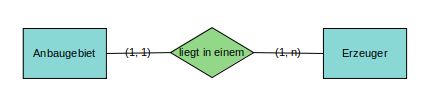
\includegraphics[width=14cm]{images/16.png}
	\caption{Beziehung zwischen den \textit{Entity-Typen} Anbaugebiet und Erzeuger aus dem Weingut Testmodell}
	\label{ergebnis9}
\end{figure}
\hon{}
\noindent
Die komplexeste Form bei der Erstellung von \textit{ERDs} ist ein \textit{Super-Sub-Beziehungstyp}, der als gleichschenkliges Dreieck dargestellt wird. Der Aufbau der \textit{XML-Elemente} sieht für diese Form wie folgt aus:
\begin{verbatim}
Element: draw:page
|
+-- Element: draw:custom-shape
    |
    +-- Attribut: draw:style-name
    +-- Attribut: draw:text-style-name
    +-- Attribut: draw:id
    +-- Attribut: draw:layer
    +-- Attribut: svg:width
    +-- Attribut: svg:height
    +-- Attribut: svg:x
    +-- Attribut: svg:y
    +-- Element: draw:enhanced-geometry
        |
        +-- Attribut: svg:viewBox
        +-- Attribut: draw:mirror-horizontal
        +-- Attribut: draw:mirror-vertical
        +-- Attribut: draw:type
        +-- Attribut: draw:enhanced-path
        +-- Attribut: svg:glue-points
        +-- Element: draw:equation
            |
            +-- Attribut: draw:name
            +-- Attribut: draw:formula

\end{verbatim}	

\noindent
\hon{}
\\
\noindent
Das \textit{XML-Element} \verb|draw:equation| wird dabei achtmal verwendet. (siehe Tabelle \ref{tbl:beispieltabelle9})

\begin{table}[H]
	\centering
	\begin{tabular}{lll}
		\textbf{Element} & \textbf{Wert von draw:name}  & \textbf{Wert von draw:formula} \\
		\\
		Erstes Element \verb|draw:equation| & \verb|f0|           & \verb|$0|              \\
		Zweites Element \verb|draw:equation| & \verb|f1|      & \verb|$0 /2|            \\
		Drittes Element \verb|draw:equation| & \verb|f2|       & \verb|?f1 +10800|             \\
		Viertes Element \verb|draw:equation| & \verb|f3|       & \verb|$0 *2/3|             \\
		Fünftes Element \verb|draw:equation| & \verb|f4|       & \verb|?f3 +7200|             \\
		Sechstes Element \verb|draw:equation| & \verb|f5|       & \verb|21600-?f0|             \\
		Siebtes Element \verb|draw:equation| & \verb|f6|       & \verb|?f5 /2|             \\
		Achtes Element \verb|draw:equation| & \verb|f7|       & \verb|21600-?f6|             \\
		\\
	\end{tabular}
	
	\caption{Werte von den draw:equation Elementen}
	\label{tbl:beispieltabelle9}
	
\end{table}
\noindent
\hon{}
\\
\noindent
Ein \textit{Super-Sub-Beziehungstyp} mit den Werten aus Tabelle \ref{tbl:beispieltabelle9} wird in Abbildung \ref{ergebnis9} gezeigt.
\\
\noindent
Falls der \textit{Beziehungstyp} \textit{disjunkt} ist, bekommt der Maximalwert der Beziehung zu dem \textit{Super-Typen} den Wert \verb|1| und das Dreieck ist \textit{weiß} gefüllt.
Falls der \textit{Beziehungstyp} \textit{nicht disjunkt} ist, bekommt der Maximalwert der Beziehung zu dem \textit{Super-Typen} den Wert der Anzahl der \textit{Sub-Typen} und das Dreieck ist \textit{schwarz} gefüllt.
\\
\\
\noindent
Falls der \textit{Beziehungstyp} \textit{total} ist, bekommt der Minimalwert der Beziehung zu dem \textit{Super-Typen} den Wert \verb|1| und der \textit{Konnektor} zu dem \textit{Super-Typ} ist strichliert, da die eigentliche Darstellung mit zwei parallel verlaufenden Linien unter \textit{Draw} nicht möglich ist.
Falls der \textit{Beziehungstyp} \textit{partiell} ist, bekommt der Minimalwert des \textit{Konnektors} zu dem \textit{Super-Typen} den Wert \verb|0| und der \textit{Konnektor} zu dem \textit{Super-Typ} ist durchgezogen.	
Die \textit{Beziehungskardinalität} zu den \textit{Sub-Typen} ist immer \verb|(1, 1)|.

\begin{figure}[H]
	\centering
	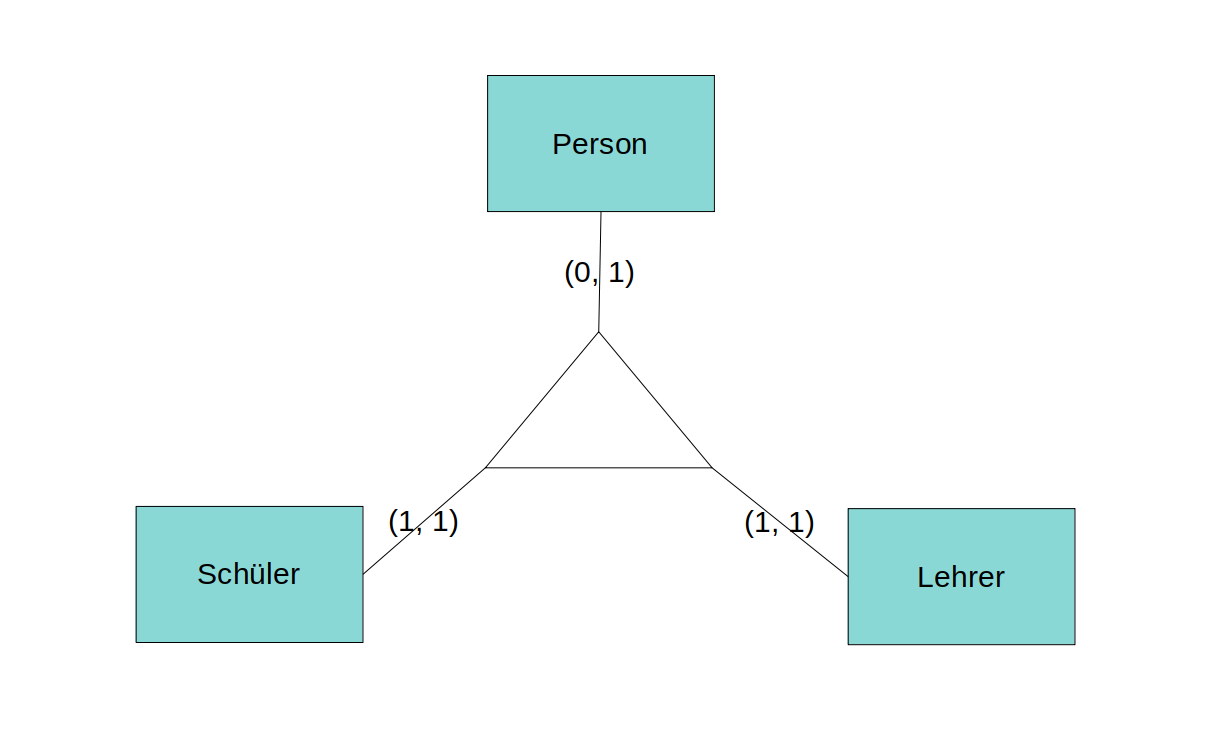
\includegraphics[width=12cm]{images/17.png}
	\caption{\textit{Disjunkter} und \textit{partieller} \textit{Super-Sub-Beziehungstyp} erstellt mit den Werten aus Tabelle \ref{tbl:beispieltabelle9} angewendet auf das Testmodell SIS}
	\label{ergebnis9}
\end{figure}
\noindent
\hon{}
\\
\noindent
\textit{Abhängige Entity-Typen} und \textit{Identifizierende Beziehungstypen} werden mit einer doppelten Umrahmung dargestellt. Dafür werden zwei Rechtecke in das \textit{XML-Element} \verb|draw:g| als \textit{XML-Kindelemente} eingefügt. Die Breite und Höhe des zusätzlichen Rechtecks beträgt 9 cm beziehungsweise 5 cm. Zusätzlich sind die x- und y-Koordinate um 0.5 cm zu verschoben, um den Abstand zwischen den beiden Rechtecken auf jeder Seite gleich zu halten. Ein \textit{abhängiger Entity-Typ} könnte in dem Dateiformat \textit{FODG} wie folgt aussehen:

\begin{verbatim}
<draw:g draw:style-name="gr7" draw:id="kveranst">
    <draw:custom-shape draw:style-name="gr1" draw:text-style-name="P8" 
          draw:layer="layout" svg:width="10cm" svg:height="6cm" 
          svg:x="130.0cm" svg:y="32.62cm">
        <text:p text:style-name="P1">
             <text:span text:style-name="T1"/>
        </text:p>
        <draw:enhanced-geometry svg:viewBox="0 0 21600 21600" 
              draw:mirror-horizontal="false" draw:mirror-vertical="false" 
              draw:type="rectangle" 
              draw:enhanced-path="M 0 0 L 21600 0 21600 21600 0 21600 0 0 Z N"/>
    </draw:custom-shape>
    <draw:custom-shape draw:style-name="gr_ent" 
          draw:text-style-name="P_ent" draw:id="kveranst" 
          draw:layer="layout" svg:width="9cm" svg:height="5cm" 
          svg:x="130.5cm" svg:y="33.12cm">
        <text:p text:style-name="P1">
             <text:span text:style-name="T6">kveranst</text:span>
        </text:p>
        <draw:enhanced-geometry svg:viewBox="0 0 21600 21600" 
              draw:mirror-horizontal="false" draw:mirror-vertical="false" 
              draw:type="rectangle" 
              draw:enhanced-path="M 0 0 L 21600 0 21600 21600 0 21600 0 0 Z N"/>
    </draw:custom-shape>
</draw:g>
\end{verbatim} 
\noindent
\hon{}
\\
\noindent
Das \textit{Primary-Key-Attribut} des \textit{abhängigen Entity-Typen} wird strichliert unterstrichen.
Dafür benötigen die \textit{XML-Attribute} aus Tabelle \ref{tbl:beispieltabelle9} jene Werte, falls das Darstellen in Farbe erwünscht ist.

\begin{table}[H]
	\centering
	\begin{tabular}{lll}
		\textbf{Element} & \textbf{Attribut}  & \textbf{Wert} \\
		\\
		draw:custum-shape des äußeren Rechtecks & draw:style-name           & gr1             \\
		draw:custum-shape des äußeren Rechtecks & draw:text-style-nam      & P8            \\
		text:p des äußeren Rechtecks & text:style-name       & P1             \\
		text:span des äußeren Rechtecks & text:style-name       & T1             \\
		draw:custum-shape des inneren Rechtecks & draw:style-name           & gr-ent             \\
		draw:custum-shape des inneren Rechtecks & draw:text-style-nam      & P-ent            \\
		text:p des inneren Rechtecks & text:style-name       & P1             \\
		text:span des inneren Rechtecks & text:style-name       & T6             \\
		\\
	\end{tabular}
	
	\caption{Tabelle der \textit{XML-Attributwerte} um \textit{Primary-Key-Attribute} von \textit{abhängigen Entity-Typen} in Farbe darzustellen}
	\label{tbl:beispieltabelle9}
	% Verweis im Text mittels \ref{tbl:beispieltabelle}
	
\end{table}
\noindent
\hon{}
\\
\noindent
Ist die Darstellung in Farbe nicht erwünscht ist, bekommen die \textit{XML-Attribute} die Werte aus Tabelle \ref{tbl:beispieltabelle10}. 

\begin{table}[H]
	\centering
	\begin{tabular}{lll}
		\textbf{Element} & \textbf{Attribut}  & \textbf{Wert} \\
		\\
		draw:custum-shape des äußeren Rechtecks & draw:style-name           & gr1             \\
		draw:custum-shape des äußeren Rechtecks & draw:text-style-nam      & P8            \\
		text:p des äußeren Rechtecks & text:style-name       & P1             \\
		text:span des äußeren Rechtecks & text:style-name       & T1             \\
		draw:custum-shape des inneren Rechtecks & draw:style-name           & gr1             \\
		draw:custum-shape des inneren Rechtecks & draw:text-style-nam      & P8            \\
		text:p des inneren Rechtecks & text:style-name       & P1             \\
		text:span des inneren Rechtecks & text:style-name       & T1             \\
		\\
	\end{tabular}
	
	\caption{Tabelle der \textit{XML-Attributwerte} um \textit{Primary-Key-Attribute} von \textit{abhängigen Entity-Typen} farblos darzustellen}
	\label{tbl:beispieltabelle10}
	% Verweis im Text mittels \ref{tbl:beispieltabelle}
	
\end{table}	


\noindent
\hon{}
\\
\noindent
Die Abbildung \ref{ergebnis10} zeigt einen \textit{identifizierenden Beziehungstyp} und einen \textit{abhängigen Entity-Typen} mit dessen \textit{Primary-Key-Attribut}.


\begin{figure}[H]
	\centering
	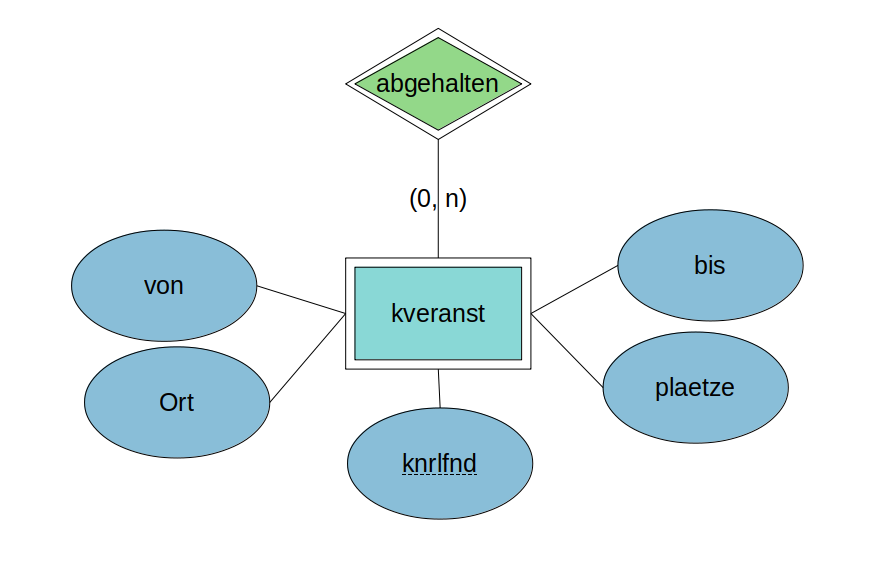
\includegraphics[width=12cm]{images/18.png}
	\caption{\textit{Identifizierender Beziehungstyp} und ein \textit{abhängigen Entity-Typ} mit dessen \textit{Primary-Key-Attribut}}
	\label{ergebnis10}
\end{figure}	

\subsubsubsection{IDs}
\hon{}

\noindent
Eine zentrale Rolle in der Generierung von \textit{ERDs} über das Dateiformat spielen die IDs der Formen. Ohne diese wäre es nicht möglich \textit{Konnektoren} an \textit{Entity-Typen}, \textit{Attributen} oder \textit{Beziehungstypen} zu verankern. Da eine ID eindeutig sein muss, reicht der Name eines \textit{Attributes} oder eines \textit{Beziehungstyps} meist nicht aus, da dieser meist öfter als einmal vorkommen kann. Aus diesem Grund werden die IDs aus mehreren Faktoren zusammengesetzt:
\begin{itemize}
	\item Die ID eines \textit{Entity-Typs} ist dessen Name. Dieser muss eindeutig sein und reicht daher aus.
	\item Die ID eines Attributs setzt sich aus dem Namen des zugehörigen \textit{Entity-Typs} und dem Namen des Attributs zusammen.
	\item Die ID eines \textit{Beziehungstyps} ist dessen Name. Dieser muss eindeutig sein und reicht daher aus.
	\item Die ID eines \textit{Beziehungsattributs} setzt sich aus dem Namen der zugehörigen Beziehung und dem Namen des Attributs zusammen.
	\item Die ID einer \textit{Super-Sub-Beziehung} setzt sich aus dem Namen der \textit{Super-Sub-Beziehung} und dem Suffix \textit{super-sub} zusammen.
\end{itemize} 


\subsubsubsection{Vor- und Nachteile}
\hon{}
\\
\noindent
Die Erstellung eines \textit{ERDs} in \textit{LibreOffice Draw} über das Dateiformat bringt folgende Vorteile mit sich:
\begin{itemize}
	\item Durch \textit{Reverse Engineering} lässt sich sehr schnell die Bedeutung der einzelnen \textit{XML-Elemente} und \textit{XML-Attribute} herausfinden, was ein schnelles Einlesen in das Dateiformat ermöglicht.
	\item Die Erzeugung einer \textit{XML-Datei} in \textit{Python} ist sehr performant im Vergleich zu der Verwendung der \textit{LibreOffice API} (siehe Abschnitt \ref{performance}).
\end{itemize}
\noindent
Allerdings bringt diese Variante auch einige Nachteile mit sich:
\begin{itemize}
	\item Die Modifikation des Dateiformats ist sehr heikel. Ein falsches Einrücken oder das Erzeugen eines nicht vorhandenen \textit{XML-Attributs} reicht, um die \textit{FODG}-Datei nicht mehr öffnen zu können.
	\begin{figure}[H]
		\centering
		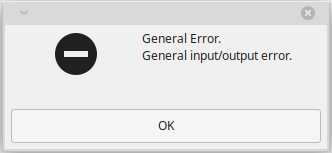
\includegraphics[width=7cm]{images/21.png}
		\caption{Fehlermeldung in \textit{LibreOffice Draw}, falls das Dateiformat ungültig ist.}
		\label{ergebnis10}
	\end{figure}
	
	\item Es gibt keine Dokumentation, in der das Dateiformat beschrieben steht.
\end{itemize}


\subsubsection{Performancevergleich}
\label{performance}
\hon{}

Bei der Generierung der Testmodelle ist ein klarer Performanceunterschied erkennbar. Um diesen Unterschied zu veranschaulichen, wurde jedes Testmodell in beiden Generierungsvarianten generiert und dabei die benötigte Zeit gemessen. Um mögliche Ausreißer zu eleminieren, wurde jedes Testmodell fünfmal pro Generierungsvariante generiert und danach wurde der Durchschnitt gebildet. Die Testmodelle wurden in Farbe und mit Attributen generiert. Die Ergebnisse des Vergleichs sind in Tabelle \ref{tbl:performance} veranschaulicht.

\begin{table}[H]
	\centering
	\begin{tabular}{lll}
		\textbf{Testmodell} & \textbf{Benötigte Zeit API}  & \textbf{Benötigte Zeit Dateiformat} \\
		\\
		AAA & 29,61 Sekunden           & 0,52 Sekunden             \\
		Fußball & 25,02 Sekunden      & 0,31 Sekunden            \\
		Kinokette & 28,50 Sekunden       & 0,46 Sekunden           \\
		Mondial & 93,79 Sekunden       & 12,03 Sekunden             \\
		Rettungsstelles & 32,95 Sekunden           & 0,72 Sekunden             \\
		SF & 40,32 Sekunden      & 0,16 Sekunden            \\
		SIS & 29,83 Sekunden       & 0,45 Sekunden             \\
		Tankstelle & 25,99 Sekunden       & 0,36 Sekunden             \\
		Weingut & 18,86 Sekunden       & 0,15 Sekunden             \\
		\\
	\end{tabular}
	
	\caption{Benötigte Zeit jedes Testmodells in den beiden Generierungsvarianten.}
	\label{tbl:performance}
\end{table}
\noindent
\hon{}
\\

\noindent
Folgende Soft- beziehungsweise Hardware wurde für die Generierung der Testmodelle verwendet:

\begin{itemize}
	\item OS: Linux Mint virtualisiert mittels Oracle VM VirtualBox
	\item CPU: Intel Core i5-6600k @ 3,9GHz
	\item GPU: GeForce GTX 980 Ti
	\item RAM: 16GB @ 2666MHz
\end{itemize}


\subsection{Layout}
\hon{}
\noindent
Um ein aufwendiges Nachbearbeiten des \textit{ERDs} zu verhindern, wird das \textit{ERD} mit einem Layout erzeugt. Als Layoutalgorithmus wurde \textit{Graphviz} verwendet. (siehe Kapitel \ref{layout})







